\documentclass{article}

\RequirePackage[svgnames]{xcolor}
\definecolor{UTorange}{RGB}{207, 83, 0} 
\definecolor{UTwhite}{RGB}{214, 210, 196}
\definecolor{UTgray}{RGB}{51, 63, 72}

\definecolor{UCLAblue}{RGB}{39, 116, 174} 
\definecolor{UCLAdark}{RGB}{0, 59, 92}
\definecolor{UCLAlight}{RGB}{218, 235, 254}
\definecolor{UCLAgold}{RGB}{255, 209, 0}

\definecolor{mered}{HTML}{882255}
\definecolor{megreen}{HTML}{004953}
\definecolor{mepink}{HTML}{AA4499}
\definecolor{rosequartz}{HTML}{F7CAC9}
\definecolor{serenity}{HTML}{92A8D1}

\definecolor{dark-red}{rgb}{0.4,0.15,0.15}
\definecolor{dark-blue}{rgb}{0.15,0.15,0.4}
\definecolor{medium-blue}{rgb}{0,0,0.5}

\usepackage{amsmath,amssymb, enumerate, tikz-cd,mathrsfs,hyperref,colortbl,bm}
\usepackage{graphicx, animate,lmodern}
\usepackage[export]{adjustbox}
\usepackage{cleveref}

\usepackage[outline]{contour}


%\usepgfplotslibrary{external}
 % \usetikzlibrary{external}
 % \tikzexternalize[prefix=tikz/]

\usepackage{float}
\usepackage{caption}
\usepackage{tikz}
\usepackage{tikz-3dplot}
\usepackage{pgfplots}
\pgfplotsset{compat=1.18}
\usetikzlibrary{scopes, angles, quotes, arrows.meta, calc, positioning, decorations.markings, decorations.pathreplacing,bending,shapes}
\usepgfplotslibrary{colormaps,fillbetween}

\newcommand\fixthis[1]{\textcolor{red}{#1}}

\newcommand{\R}{\mathbb{R}}
\newcommand{\C}{\mathbb{C}}
\newcommand{\Z}{\mathbb{Z}}
\newcommand{\Q}{\mathbb{Q}}
\newcommand{\F}{\mathbb{F}}
\newcommand{\N}{\mathbb{N}}

%my macros
\newcommand{\Sphere}{\mathbb{S}}
\newcommand{\TatekG}{\mathsf{Tate}(kG)}
\newcommand{\kGMod}{kG$-$\mathsf{Mod}}
\newcommand{\StMod}{\mathsf{StMod}}
\newcommand{\Mod}{\mathsf{Mod}}
\newcommand{\Top}{\textnormal{Top}}
\newcommand{\D}{\mathcal{D}}
\newcommand{\Ho}{\mathsf{Ho}}
\newcommand{\Hom}{\textnormal{Hom}}
\newcommand{\Ext}{\textnormal{Ext}}
\newcommand{\Tor}{\textnormal{Tor}}
\newcommand{\Cell}{\mathsf{Cell}}
\newcommand{\End}{\mathsf{End}}
\newcommand{\Spec}{\textnormal{Spec}}
\newcommand{\holim}{\textnormal{holim}}
\newcommand{\hocolim}{\textnormal{hocolim}}
\newcommand{\1}{\mathds{1}}
\newcommand{\Supp}{\textnormal{Supp}}
\newcommand{\supp}{\textnormal{supp}}
\newcommand{\Pic}{\textnormal{Pic}}
\newcommand{\pic}{\mathfrak{pic}}
\newcommand{\gl}{\mathfrak{gl}}
\newcommand{\Tot}{\textnormal{Tot}}
\newcommand{\CAlg}{\textnormal{CAlg}}
\newcommand{\Res}{\textnormal{Res}}
\newcommand{\CoInd}{\textnormal{CoInd}}


\tikzstyle{vector}=[-Latex,very thick, mered,line cap=round]
\tikzstyle{xline}=[UCLAblue,very thick]
\tikzstyle{yzp}=[canvas is zy plane at x=0]
\tikzstyle{xzp}=[canvas is xz plane at y=-1]
\tikzstyle{xyp}=[canvas is xy plane at z=1]
\def\tick#1#2{\draw[thick] (#1) ++ (#2:0.12) --++ (#2-180:0.24)}
\def\N{100}


\makeatletter %for the smooth/tension example
\tikzset{
	on each segment/.style={
		decorate,
		decoration={
			show path construction,
			moveto code={},
			lineto code={
				\path [#1]
				(\tikzinputsegmentfirst) -- (\tikzinputsegmentlast);
			},
			curveto code={
				\path [#1] (\tikzinputsegmentfirst)
				.. controls
				(\tikzinputsegmentsupporta) and (\tikzinputsegmentsupportb)
				..
				(\tikzinputsegmentlast);
			},
			closepath code={
				\path [#1]
				(\tikzinputsegmentfirst) -- (\tikzinputsegmentlast);
			},
		},
	},
}
\makeatother

\pgfplotsset{
	colormap={mesvtcolor}{
		rgb255=(145,168,209) 
		rgb255=(247,202,201)
	}%,
%	colormap/mesvtcolor,
}


\begin{document}
	
%         \begin{tikzpicture}
%     \begin{axis}[hide axis,
%     colormap/cool,view={-10}{30}, width=15cm, axis equal image]
%         % Draw sphere (example from the pgfplots manual)
%         \addplot3[
%             surf, z buffer=sort, colormap name=mesvtcolor,, domain=0:180, domain y=0:360,
% 		samples=41, samples y=25, opacity=0.5,
% 		variable=\u, variable y=\v,
% 		point meta=u,
% 		] 
% 		({-2/15 * cos(u) * (
% 		    3*cos(v) - 30*sin(u) 
% 		  + 90 *cos(u)^4 * sin(u) 
% 		  - 60 *cos(u)^6 * sin(u)  
% 		  + 5 * cos(u)*cos(v) * sin(u))
% 		 },
% 		 {-1/15 * sin(u) * (3*cos(v) 
% 		  - 3*cos(u)^2 * cos(v) 
% 		  - 48 * cos(u)^4*cos(v) 
% 		  + 48*cos(u)^6 *cos(v) 
% 		  - 60 *sin(u) 
% 		  + 5*cos(u)*cos(v)*sin(u) 
% 		  - 5*cos(u)^3 * cos(v) *sin(u) 
% 		  - 80*cos(u)^5 * cos(v)*sin(u) 
% 		  + 80*cos(u)^7 * cos(v) * sin(u))
% 		 },
% 		 {2/15 * (3 + 5*cos(u) *sin(u))*sin(v)});
% 	\end{axis}
% \end{tikzpicture}

% \begin{tikzpicture}
%   \begin{axis}[
%     axis lines=center,
%     grid=major,
%     ymax=2,ymin=-2,
%     xtick={-(3/2)*pi,-pi, -(1/2)*pi, 0, (1/2)*pi, pi,(3/2)*pi},
%     xticklabel style={font=\footnotesize},
%     xticklabels={\contour{white}{$-\frac{3\pi}{2}$},\contour{white}{$-\pi$},\contour{white}{$-\frac{\pi}{2}$},,\contour{white}{$\frac{\pi}{2}$},\contour{white}{$\pi$},\contour{white}{$\frac{3\pi}{2}$}},
%     no marks,
%     ]
%     \addplot+[smooth,ultra thick,UCLAblue,domain=-3.14:3.14] {sin(deg(x))}; % actual curve
%     \addplot+[draw=none,name path=A] {sin(deg(x))}; % actual curve
%     \addplot+[draw=none,name path=B] {0};     % “fictional” curve
%     \addplot+[green] fill between[of=A and B,soft clip={domain=0:3.14}]; % filling
%     \addplot+[red] fill between[of=B and A,soft clip={domain=-3.14:0}]; % filling
%   \end{axis}
% \end{tikzpicture}

%     \begin{tikzpicture}
%   \begin{axis}[
%     axis lines=center,
%     grid=major,
%     ymax=3,ymin=-1,
%     xmax=1,xmin=-1,
%     % xtick={-(3/2)*pi,-pi, -(1/2)*pi, 0, (1/2)*pi, pi,(3/2)*pi},
%     % xticklabel style={font=\footnotesize},
%     % xticklabels={\contour{white}{$-\frac{3\pi}{2}$},\contour{white}{$-\pi$},\contour{white}{$-\frac{\pi}{2}$},,\contour{white}{$\frac{\pi}{2}$},\contour{white}{$\pi$},\contour{white}{$\frac{3\pi}{2}$}},
%     no marks,
%     ]
%     \addplot+[smooth,ultra thick,UCLAblue,samples=60] {1/(sqrt(1-x*x))} node[midway, above right]{$y=\frac{1}{\sqrt{1-x^2}}$} ; % actual curve
%     % \addplot+[draw=none,name path=B] {0};     % “fictional” curve
%     % \addplot+[green] fill between[of=A and B,soft clip={domain=0:3.14}]; % filling
%     % \addplot+[red] fill between[of=B and A,soft clip={domain=-3.14:0}]; % filling
%   \end{axis}
% \end{tikzpicture}

%     \begin{tikzpicture}
%   \begin{axis}[
%     axis lines=center,
%     grid=major,
%     ymax=3,ymin=-3,
%     xmax=3,xmin=-3,
%     % xtick={-(3/2)*pi,-pi, -(1/2)*pi, 0, (1/2)*pi, pi,(3/2)*pi},
%     % xticklabel style={font=\footnotesize},
%     % xticklabels={\contour{white}{$-\frac{3\pi}{2}$},\contour{white}{$-\pi$},\contour{white}{$-\frac{\pi}{2}$},,\contour{white}{$\frac{\pi}{2}$},\contour{white}{$\pi$},\contour{white}{$\frac{3\pi}{2}$}},
%     no marks,
%     ]
%     \addplot+[smooth,ultra thick, UCLAblue,samples=60,domain=0:3] {x}; % pos
%     \addplot+[smooth,ultra thick,UCLAblue,samples=60,domain=-3:0] {0} node[above left]{$f^+(x)$}; % pos
%     % \addplot+[draw=none,name path=B] {0};     % “fictional” curve
%     % \addplot+[green] fill between[of=A and B,soft clip={domain=0:3.14}]; % filling
%     % \addplot+[red] fill between[of=B and A,soft clip={domain=-3.14:0}]; % filling
%   \end{axis}
% \end{tikzpicture}

%     \begin{tikzpicture}
%   \begin{axis}[
%     axis lines=center,
%     grid=major,
%     ymax=3,ymin=-3,
%     xmax=3,xmin=-3,
%     % xtick={-(3/2)*pi,-pi, -(1/2)*pi, 0, (1/2)*pi, pi,(3/2)*pi},
%     % xticklabel style={font=\footnotesize},
%     % xticklabels={\contour{white}{$-\frac{3\pi}{2}$},\contour{white}{$-\pi$},\contour{white}{$-\frac{\pi}{2}$},,\contour{white}{$\frac{\pi}{2}$},\contour{white}{$\pi$},\contour{white}{$\frac{3\pi}{2}$}},
%     no marks,
%     ]
%     \addplot+[smooth,ultra thick,mered,samples=60,domain=-3:0] {-x} node[above right]{$f^-(x)$}; % neg    
%     \addplot+[smooth,ultra thick,mered,samples=60,domain=0:3] {0}; % pos
%     % \addplot+[draw=none,name path=B] {0};     % “fictional” curve
%     % \addplot+[green] fill between[of=A and B,soft clip={domain=0:3.14}]; % filling
%     % \addplot+[red] fill between[of=B and A,soft clip={domain=-3.14:0}]; % filling
%   \end{axis}
% \end{tikzpicture}

% \begin{tikzpicture}
%   \begin{axis}[
%     axis lines=center,
%     grid=major,
%     ymax=4,ymin=-1,
%     xmax=5,xmin=-1,
%     % xtick={-(3/2)*pi,-pi, -(1/2)*pi, 0, (1/2)*pi, pi,(3/2)*pi},
%     % xticklabel style={font=\footnotesize},
%     % xticklabels={\contour{white}{$-\frac{3\pi}{2}$},\contour{white}{$-\pi$},\contour{white}{$-\frac{\pi}{2}$},,\contour{white}{$\frac{\pi}{2}$},\contour{white}{$\pi$},\contour{white}{$\frac{3\pi}{2}$}},
%     no marks,
%     ]
%     \addplot+[smooth,ultra thick, UCLAblue,domain=2:5,samples=40] {0.6*x};
%     \addplot+[smooth,ultra thick, UCLAblue,domain=2:5,samples=40] {3};
%     \addplot+[draw=none,name path=A] {3}; % actual curve
%     \addplot+[draw=none,name path=B] {0.6*x};     % “fictional” curve
%     \addplot+[UCLAgold] fill between[of=A and B,soft clip={domain=2:5}]; % filling
%     \addplot+[mered,ultra thick] (2,1.2) -- (2,3); % vertical line
%   \end{axis}
% \end{tikzpicture}

% \begin{tikzpicture}
%   \begin{axis}[
%     axis lines=center,
%     grid=major,
%     ymax=4,ymin=-1,
%     xmax=5,xmin=-1,
%     % xtick={-(3/2)*pi,-pi, -(1/2)*pi, 0, (1/2)*pi, pi,(3/2)*pi},
%     % xticklabel style={font=\footnotesize},
%     % xticklabels={\contour{white}{$-\frac{3\pi}{2}$},\contour{white}{$-\pi$},\contour{white}{$-\frac{\pi}{2}$},,\contour{white}{$\frac{\pi}{2}$},\contour{white}{$\pi$},\contour{white}{$\frac{3\pi}{2}$}},
%     no marks,
%     ]
%     \addplot+[smooth,ultra thick, UCLAblue,domain=0:2,samples=40] {0.6*x};
%     \addplot+[smooth,ultra thick, UCLAblue,domain=0:2,samples=40] {1.5*x};
%     \addplot+[draw=none,name path=B] {0.6*x};     % “fictional” curve
%     \addplot+[draw=none,name path=C] {1.5*x};     % “fictional” curve
%     \addplot+[UCLAgold] fill between[of=C and B,soft clip={domain=0:2}]; % filling
%     \addplot+[mered,ultra thick] (2,1.2) -- (2,3); % vertical line
%   \end{axis}
% \end{tikzpicture}

% \begin{tikzpicture}
%   \begin{axis}[
%     axis lines=center,
%     grid=major,
%     ymax=4,ymin=-1,
%     xmax=5,xmin=-1,
%     % xtick={-(3/2)*pi,-pi, -(1/2)*pi, 0, (1/2)*pi, pi,(3/2)*pi},
%     % xticklabel style={font=\footnotesize},
%     % xticklabels={\contour{white}{$-\frac{3\pi}{2}$},\contour{white}{$-\pi$},\contour{white}{$-\frac{\pi}{2}$},,\contour{white}{$\frac{\pi}{2}$},\contour{white}{$\pi$},\contour{white}{$\frac{3\pi}{2}$}},
%     no marks,
%     ]
%     \addplot+[smooth,ultra thick, UCLAblue,domain=0:5,samples=40] {0.6*x};
%     \addplot+[smooth,ultra thick, UCLAblue,domain=2:5,samples=40] {3};
%     \addplot+[smooth,ultra thick, UCLAblue,domain=0:2,samples=40] {1.5*x};  
%     \addplot+[draw=none,name path=A] {3}; % actual curve
%     \addplot+[draw=none,name path=B] {0.6*x};     % “fictional” curve
%     \addplot+[draw=none,name path=C] {1.5*x};     % “fictional” curve
%     \addplot+[UCLAgold] fill between[of=A and B,soft clip={domain=2:5}]; % filling
%     \addplot+[UCLAgold] fill between[of=C and B,soft clip={domain=0:2}]; % filling
%     % \addplot+[red] fill between[of=B and A,soft clip={domain=-3.14:0}]; % filling
%   \end{axis}
% \end{tikzpicture}   

% \begin{tikzpicture}
%   \begin{axis}[
%     axis lines=center,
%     grid=major,
%     ymax=1.5,ymin=-.5,
%     xmax=3,xmin=0,
%     % xtick={-(3/2)*pi,-pi, -(1/2)*pi, 0, (1/2)*pi, pi,(3/2)*pi},
%     % xticklabel style={font=\footnotesize},
%     % xticklabels={\contour{white}{$-\frac{3\pi}{2}$},\contour{white}{$-\pi$},\contour{white}{$-\frac{\pi}{2}$},,\contour{white}{$\frac{\pi}{2}$},\contour{white}{$\pi$},\contour{white}{$\frac{3\pi}{2}$}},
%     no marks,
%     ]
%     \addplot[smooth,ultra thick, UCLAblue,samples=40] {ln(x)} node[midway, above left]{$x=e^y$};
%     \addplot[smooth,ultra thick, mered,domain=1:3,samples=40] {ln(x)*ln(x)} node[midway, below right]{$x=e^{\sqrt{y}}$};
%     \addplot[draw=none,samples=40,name path=A] {ln(x)}; % actual curve
%     \addplot[draw=none,samples=40,name path=B] {ln(x)*ln(x)};     % “fictional” curve
%     \addplot[UCLAgold] fill between[of=A and B,soft clip={domain=1:2.7}]; 
%   \end{axis}
% \end{tikzpicture}


%	\begin{tikzpicture}
%		\pgfset{declare function={f(\x)=3*exp(-(\x))*(\x)^3+1;}}
%		\begin{axis}[
%			domain=0:8.1,
%			samples=100,
%			axis lines=middle,
%			ymax=5.5,
%			]
%			\addplot [
%			mered,fill=mered!10,
%			integral segments=16,
%			integral min=0:8
%			] {f(x)};
%			\addplot [ultra thick, UCLAblue] {f(x)};
%		\end{axis}
%	\end{tikzpicture}


%	\begin{tikzpicture} 
%		\pgfset{declare function={f(\x)=3*exp(-(\x))*(\x)^3+1;}}
%		\begin{axis}[
%			domain=0:8.1,
%			samples=100,
%			axis lines=middle,
%			ymax=5.5,
%			]					
%			\addplot [
%			megreen,fill=megreen!10,
%			integral segments=16,
%			integral max=0:8
%			] {f(x)};
%			\addplot [ultra thick, UCLAblue] {f(x)};
%		\end{axis}
%	\end{tikzpicture}
	
%	\begin{tikzpicture}
%		\pgfset{declare function={f(\x)=3*exp(-(\x))*(\x)^3+1;}}
%		\begin{axis}[
%			domain=0:8.1,
%			samples=100,
%			axis lines=middle,
%			ymax=5.5,
%			]
%			\addplot [
%			megreen,fill=rosequartz!50,
%			integral segments=16,
%			integral max=0:8
%			] {f(x)};
%			\addplot [
%			megreen,fill=white,
%			integral segments=16,
%			integral min=0:8
%			] {f(x)};
%			\addplot [ultra thick, UCLAblue] {f(x)};
%		\end{axis}
%	\end{tikzpicture}	

%	\begin{tikzpicture}
%		\pgfset{declare function={f(\x)=3*exp(-(\x))*(\x)^3+1;}}
%		\begin{axis}[
%			domain=0:8.1,
%			samples=100,
%			axis lines=middle,
%			ymax=5.5,
%			]
%			\addplot [
%			mered,fill=mered!10,
%			integral segments=32,
%			integral min=0:8
%			] {f(x)};
%			\addplot [ultra thick, UCLAblue] {f(x)};
%		\end{axis}
%	\end{tikzpicture}


%	\begin{tikzpicture} 
%		\pgfset{declare function={f(\x)=3*exp(-(\x))*(\x)^3+1;}}
%		\begin{axis}[
%			domain=0:8.1,
%			samples=100,
%			axis lines=middle,
%			ymax=5.5,
%			]					
%			\addplot [
%			megreen,fill=megreen!10,
%			integral segments=32,
%			integral max=0:8
%			] {f(x)};
%			\addplot [ultra thick, UCLAblue] {f(x)};
%		\end{axis}
%	\end{tikzpicture}
%
	% \begin{tikzpicture}
	% 	\pgfset{declare function={f(\x)=3*exp(-(\x))*(\x)^3+1;}}
	% 	\begin{axis}[
	% 		domain=0:8.1,
	% 		samples=100,
	% 		axis lines=middle,
	% 		ymax=5.5,
	% 		]
	% 		\addplot [
	% 		megreen,fill=rosequartz!50,
	% 		integral segments=32,
	% 		integral max=0:8
	% 		] {f(x)};
	% 		\addplot [
	% 		megreen,fill=white,
	% 		integral segments=16,
	% 		integral min=0:8
	% 		] {f(x)};
	% 		\addplot [ultra thick, UCLAblue] {f(x)};
	% 	\end{axis}
	% \end{tikzpicture}	

%	\begin{tikzpicture}
%		\begin{axis}[
%			axis lines=center,
%			grid=major,
%			ymax=1.5,ymin=-.5,
%			xmax=1.5,xmin=-.5,
%			% xtick={-(3/2)*pi,-pi, -(1/2)*pi, 0, (1/2)*pi, pi,(3/2)*pi},
%			% xticklabel style={font=\footnotesize},
%			% xticklabels={\contour{white}{$-\frac{3\pi}{2}$},\contour{white}{$-\pi$},\contour{white}{$-\frac{\pi}{2}$},,\contour{white}{$\frac{\pi}{2}$},\contour{white}{$\pi$},\contour{white}{$\frac{3\pi}{2}$}},
%			no marks,
%			]
%			\addplot+[smooth,ultra thick, UCLAblue,domain=0:1,samples=40] {1-x*x}  node[midway,above right]{$y=1-x^2$};
%			\addplot+[draw=none,samples=40,name path=A] {1-x*x}; % actual curve
%			\addplot+[draw=none,name path=B] {0};     % “fictional” curve
%			\addplot+[UCLAgold] fill between[of=A and B,soft clip={domain=0:1}]; % filling
%			% \addplot+[red] fill between[of=B and A,soft clip={domain=-3.14:0}]; % filling
%		\end{axis}
%	\end{tikzpicture}

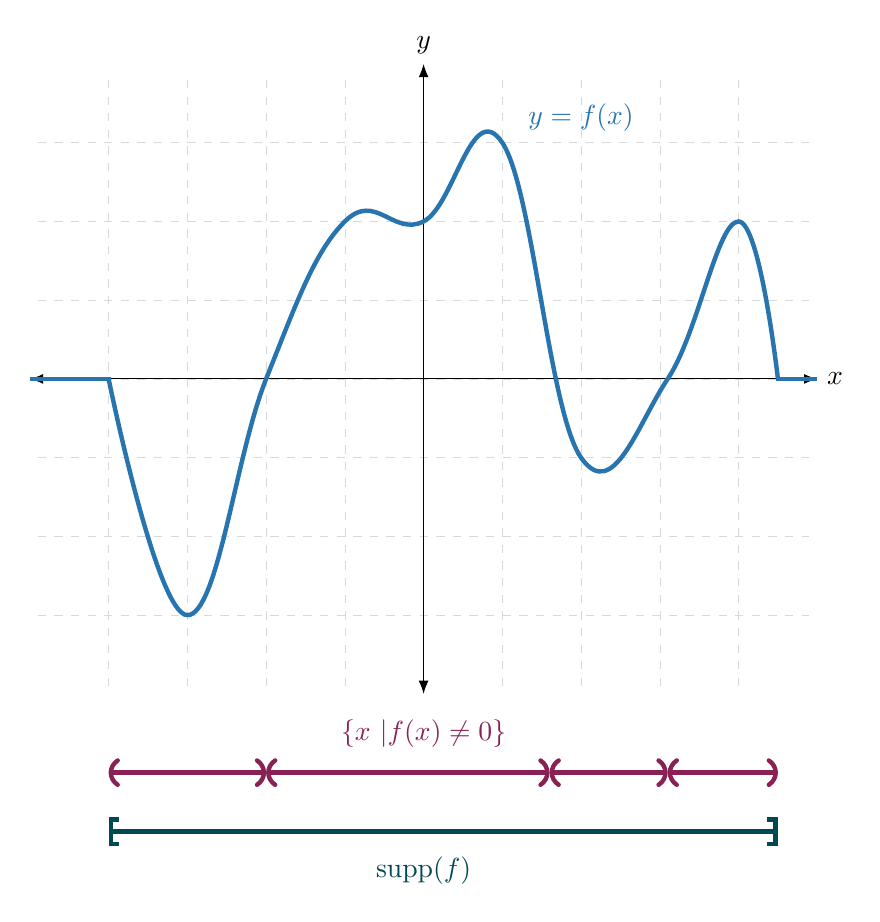
\begin{tikzpicture}
	\draw[help lines, color=gray!30, dashed] (-4.9,-3.9) grid (4.9,3.9);
	\draw[Latex-Latex] (-5,0)--(5,0) node[right]{$x$};
	\draw[Latex-Latex] (0,-4)--(0,4) node[above]{$y$};
	\draw[color=UCLAblue, ultra thick]  plot[smooth, tension=.7] coordinates {(-4,0) (-3,-3) (-2,0) (-1,2) (0,2) (1,3) (2,-1) (3.1,0) (4,2) (4.5,0)};
	\draw[color=UCLAblue, ultra thick]  plot[smooth] coordinates {(-5,0) (-3.97,0)};
	\draw[color=UCLAblue, ultra thick]  plot[smooth] coordinates {(4.47,0) (5,0)};
	\draw[color=UCLAblue, ultra thick] (2,3) node[above]{$y = f(x)$};
	\draw[color=mered, ultra thick, (-)] (-4,-5) -- (-2,-5);
	\draw[color=mered, ultra thick, (-)] (-2,-5) -- (1.6,-5);
	\draw[color=mered, ultra thick, (-)] (1.6,-5) -- (3.1,-5);
	\draw[color=mered, ultra thick, (-)] (3.1,-5) -- (4.5,-5);
	\draw[color=mered, ultra thick] (0,-4.5) node{$\{x \ | f(x) \neq 0 \}$};
	\draw[color=megreen, ultra thick, {[-]}] (-4,-5.75) -- (4.5,-5.75);
	\draw[color=megreen, ultra thick] (0,-6.25) node{$\textnormal{supp}(f)$};
\end{tikzpicture}


%\begin{tikzpicture}
%	\draw[xstep=.2,ystep=.5,lightgray,ultra thin] (-1.1,-1.5) grid (1.1,1.5);
%	\draw[Latex-Latex] (-1.1,0) -- (1.1,0) node[right] {$x$};
%	\draw[Latex-Latex] (0,-1) -- (0,1.1) node[above] {$y$};
%	\draw[UCLAblue,domain=0.01:1,samples=5000] plot (\x, {sin((1/\x)r)});	
%	\draw[UCLAblue,domain=-1:-0.01,samples=5000] plot (\x, {sin((1/\x)r)});
%\end{tikzpicture}  
	
	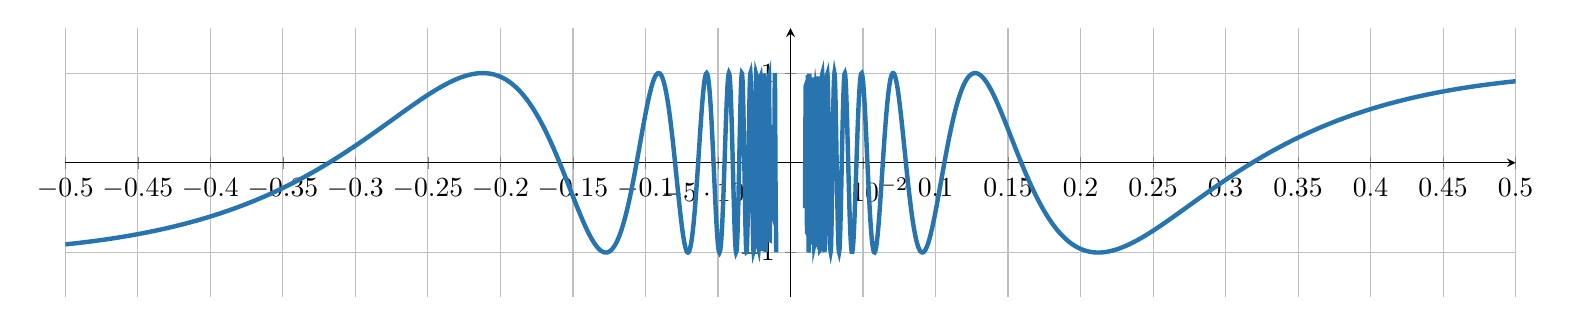
\begin{tikzpicture}
		\begin{axis}[
			axis lines=center,
			grid=major,
			ymax=1.5,ymin=-1.5,
			xmax=.5,xmin=-.5,
			width=20cm,
			height=5cm,
			% xtick={-(3/2)*pi,-pi, -(1/2)*pi, 0, (1/2)*pi, pi,(3/2)*pi},
			% xticklabel style={font=\footnotesize},
			% xticklabels={\contour{white}{$-\frac{3\pi}{2}$},\contour{white}{$-\pi$},\contour{white}{$-\frac{\pi}{2}$},,\contour{white}{$\frac{\pi}{2}$},\contour{white}{$\pi$},\contour{white}{$\frac{3\pi}{2}$}},
			no marks,
			]
			\addplot+[smooth,ultra thick,UCLAblue,domain=0.01:1,samples=2000] {sin(deg(1/x))}; % pos   
			\addplot+[smooth,ultra thick,UCLAblue,domain=-1:-0.01,samples=2000] {sin(deg(1/x))}; % neg
		\end{axis}
	\end{tikzpicture}	

	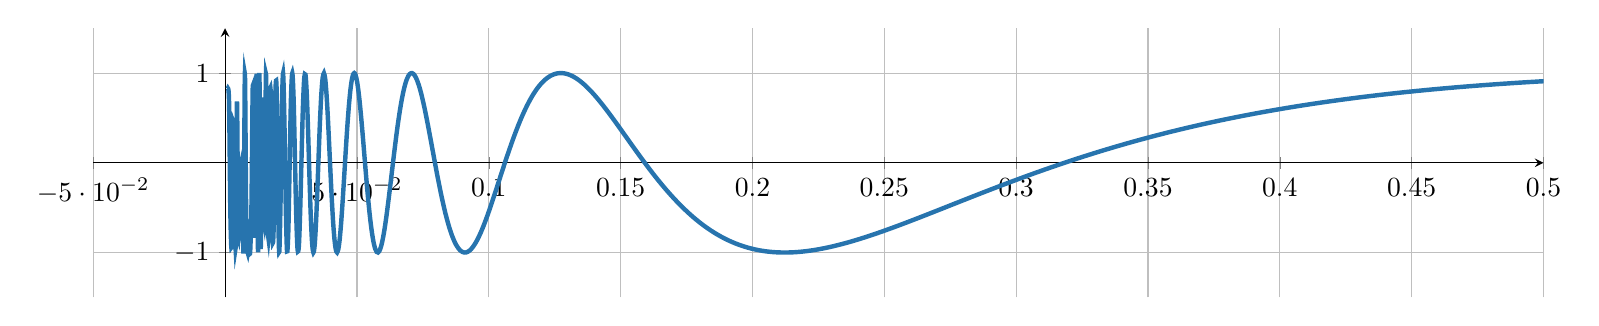
\begin{tikzpicture}
		\begin{axis}[
			axis lines=center,
			grid=major,
			ymax=1.5,ymin=-1.5,
			xmax=.5,xmin=-.05,
			width=20cm,
			height=5cm,
			% xtick={-(3/2)*pi,-pi, -(1/2)*pi, 0, (1/2)*pi, pi,(3/2)*pi},
			% xticklabel style={font=\footnotesize},
			% xticklabels={\contour{white}{$-\frac{3\pi}{2}$},\contour{white}{$-\pi$},\contour{white}{$-\frac{\pi}{2}$},,\contour{white}{$\frac{\pi}{2}$},\contour{white}{$\pi$},\contour{white}{$\frac{3\pi}{2}$}},
			no marks,
			]
			\addplot+[smooth,ultra thick,UCLAblue,domain=0.001:1,samples=2000] {sin(deg(1/x))}; % pos   
		\end{axis}
	\end{tikzpicture}	

 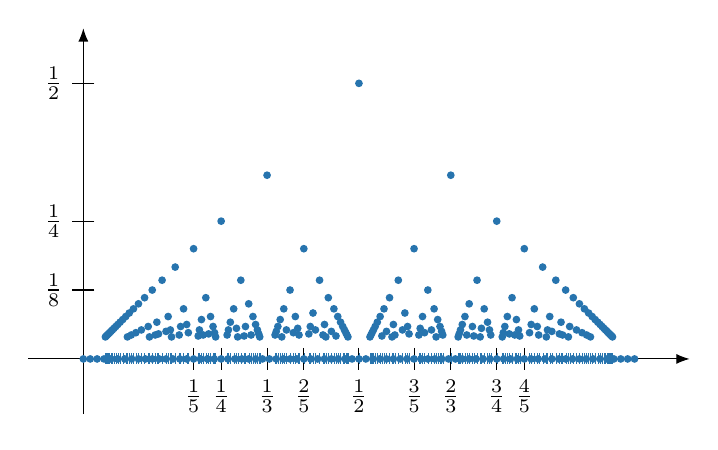
\begin{tikzpicture}[scale=7]
\draw [-Latex] (-0.1,0) -- (1.1,0);
\draw [-Latex] (0,-0.1) -- (0,0.6);
\draw (0.02,1/2) -- (-0.02,1/2) node[left,xshift={(-(1+pow(-1,1)))*3pt}]{$\frac{1}{2}$};
\draw (0.02,1/4) -- (-0.02,1/4) node[left,xshift={(-(1+pow(-1,1)))*3pt}]{$\frac{1}{4}$};
\draw (0.02,1/8) -- (-0.02,1/8) node[left,xshift={(-(1+pow(-1,1)))*3pt}]{$\frac{1}{8}$};
\foreach \X in {1,...,8}
{\ifnum\X=1
\else
%\draw (0.02,1/\X) -- (-0.02,1/\X) node[left,xshift={(-(1+pow(-1,\X)))*5pt}]{$\frac{1}{\X}$};
\fi
}
\foreach \X [evaluate=\X as \Ymax using {int(\X-1)}]in {25,24,...,2}
{\foreach \Y in {1,...,\Ymax}
 {\ifnum\X<6
 \draw (\Y/\X,0.02) -- (\Y/\X,-0.02) node[below,fill=white]{$\frac{\Y}{\X}$};
 \else
 \draw[ultra thin, UCLAblue] (\Y/\X,0.01) -- (\Y/\X,-0.01);
 \fi
 \pgfmathtruncatemacro{\TST}{gcd(\X,\Y)}
 \ifnum\TST=1
 \fill[UCLAblue] ({\Y/\X},1/\X) circle(0.2pt); 
 \fi
 }
}
\foreach \X in {0,1,...,80}
{\fill[UCLAblue] (\X/80,0) circle(0.2pt); }
\end{tikzpicture}
 
\end{document}